\begin{frame}{What is Deep Unsupervised Learning?}
    \textbf{Deep Unsupervised Learning} aims to discover \textbf{hidden patterns} and \textbf{structures} in raw data using deep neural networks, \textbf{without any human-provided labels}. 
    
    It focuses on \textbf{capturing rich patterns in raw data with deep networks in a label-free way}.
        \begin{itemize}
            \item \textbf{Learns from observation} --- mimics how humans learn from experience
            \item \textbf{Discovers structure} --- finds groups, similarities, and representations
            \item \textbf{Scales to complex data} --- uses deep models to capture abstract features
            \item \textbf{Generative Models} --- recreate raw data distribution
            \item \textbf{Self-supervised Learning} --- “puzzle” tasks that require semantic understanding
        \end{itemize}
        \vspace{0.5em}
        \centering
        {\Large \textbf{Why do we care?}}
\end{frame}

\begin{frame}{}
    \begin{center}
    \begin{minipage}{0.9\textwidth}
        \begin{columns}
            \column{0.2\textwidth}
                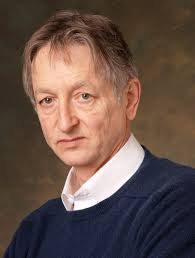
\includegraphics[width=0.8\linewidth]{images/dul/slide_15_1_img.png}
            \column{0.5\textwidth}
                \centering
                \textbf{Geoffrey Hinton}\\
                (in his 2014 AMA on Reddit)
        \end{columns}
        \vspace{1em}
        \begin{center}
        \textit{“The brain has about $10^{14}$ synapses and we only live for about $10^{9}$ seconds. 
        So we have a lot more parameters than data. This motivates the idea that we must do a lot of 
        unsupervised learning since the perceptual input (including proprioception) is the only place 
        we can get $10^{5}$ dimensions of constraint per second.”}
        \end{center}
    \end{minipage}
    \end{center}
\end{frame}

\begin{frame}{}
    \begin{columns}
        \column{0.3\textwidth}
            \centering
            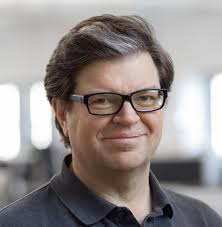
\includegraphics[width=0.8\linewidth]{images/dul/slide_16_2_img.png}
            \textbf{Yann LeCun}\\[1em]
            \textcolor{blue}{Need tremendous amount of information to build machines that have common sense and generalize well.}\\[1em]
            [LeCun-20161205-NeurIPS-keynote]
        \column{0.7\textwidth}
            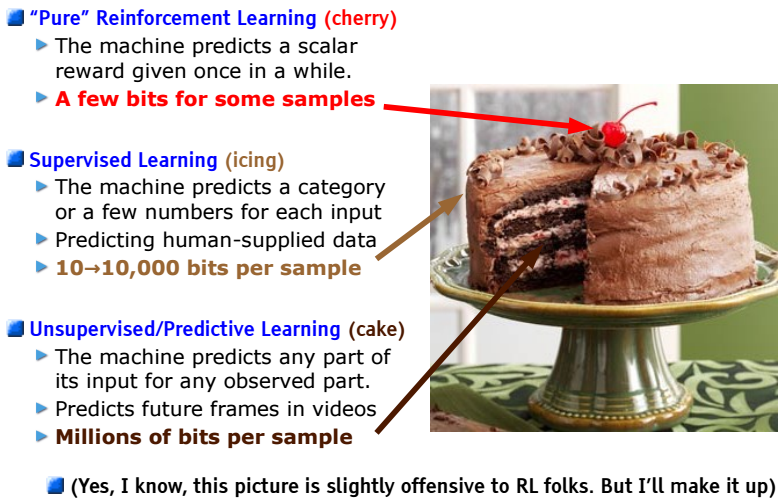
\includegraphics[width=1.05\linewidth]{images/dul/slide_16_1_img.png}
    \end{columns}
\end{frame}

\begin{frame}{``Ideal Intelligence``}
    \begin{itemize}
        \item \textbf{“Ideal Intelligence” is all about compression} (finding all patterns)
        \item Finding all patterns = short description of raw data (\textit{low Kolmogorov Complexity})
        \item Shortest code-length = optimal inference (\textit{Solomonoff Induction})
        \item Extensible to optimal action-making agents (\textit{AIXI})
    \end{itemize}
    \vspace{1em}
    \textbf{Transfer Learning via Compression:}
    \begin{itemize}
        \item Assume we pretrain unsupervised on Data Distribution $D_1$ and then finetune on Data Distribution $D_2$
        \item If $D_1$ and $D_2$ are related, compressing $D_2$ conditioned on $D_1$ should be more efficient than compressing $D_2$ outright
        \item \textbf{Hence:} pretraining on $D_1$ should aid faster learning of $D_2$
    \end{itemize}
\end{frame}